\documentclass[conference,compsoc]{IEEEtran}
\usepackage[T1]{fontenc}
\usepackage{amsmath,amssymb,amsthm}
\usepackage{graphicx,booktabs,array,multirow}
\usepackage[table]{xcolor}
\usepackage{url}
\definecolor{TableHead}{HTML}{FFFFFF}
\definecolor{TableBlue}{HTML}{FFFFFF}
\definecolor{LeakHigh}{rgb}{0.91333,0.53333,0.53333}
\definecolor{LeakMidHigh}{rgb}{0.95609,0.72275,0.72275}
\definecolor{LeakMidLow}{rgb}{0.79138,0.88196,0.72548}
\definecolor{LeakLow}{rgb}{0.61412,0.85255,0.52313}
\definecolor{RecoveryDot}{HTML}{A42D2D}
\definecolor{ControlDot}{HTML}{33712A}
\setlength{\arrayrulewidth}{0.334pt}
\setlength{\doublerulesep}{1.2pt}
\newcommand{\TableTop}{\hline\hline}
\newcommand{\TableHeadRule}{\hline}
\newcommand{\TableBottom}{\hline\hline}
\newcommand{\RecDot}{\textcolor{RecoveryDot}{\(\bullet\)}}
\newcommand{\CtrlDot}{\textcolor{ControlDot}{\(\bullet\)}}
\newcommand{\RateCell}[1]{%
  \ifdim #1pt<25pt\cellcolor{LeakLow}%
  \else\ifdim #1pt<50pt\cellcolor{LeakMidLow}%
  \else\ifdim #1pt<75pt\cellcolor{LeakMidHigh}%
  \else\cellcolor{LeakHigh}\fi\fi\fi #1}
\usepackage[hidelinks,pdfauthor={},pdftitle={Fresh Shuffles, Reused Secrets: Breaking KV-Cloak with Repeated-Token Prompts}]{hyperref}
\graphicspath{{figures/}}
\newtheorem{theorem}{Theorem}
\newtheorem{proposition}[theorem]{Proposition}
\newtheorem{lemma}[theorem]{Lemma}
\newcommand{\ones}{\mathbf{1}}
\newcommand{\R}{\mathbb{R}}
\newcommand{\T}{\mathsf{T}}
\newcommand{\scheme}{KV-Cloak}
\newcommand{\diag}{\operatorname{diag}}
\newcommand{\rank}{\operatorname{rank}}
\newcommand{\Stab}{\operatorname{Stab}}
\newcommand{\argmax}{\operatorname*{arg\,max}}
\begin{document}
\title{Fresh Shuffles, Reused Secrets:\\Breaking KV-Cloak with Repeated-Token Prompts}
\author{}
\maketitle
\begin{abstract}
We show how input symmetry can neutralize fresh shuffling in \scheme{}, an NDSS 2026 defense that combines secret linear transformations, additive markers, and independently shuffled KV-cache blocks. A repeated-token text prompt makes the first-layer Value rows identical. Shuffling then changes only the marker's position: protected blocks occupy an orbit of at most $b$ states, despite $b!$ possible permutations. Rank-one differences between these states reveal an equivalent row demixer and the implementation's structured column transform. The recovered parameters transfer to other requests protected by the same secrets, exposing token multisets without recovering within-block order. We characterize this orbit, establish identification under explicit nondegeneracy conditions, and derive a query bound. Against the official implementation, the attack recovers 263,029 of 263,904 head--token evaluation instances across ten models and twelve configurations. All fifteen additional model--key epochs calibrate successfully, with model-level mean recovery between 99.34\% and 100\%. A limited study of 30 synthetic closed-set values under one key yields 77.36\% expected top-1 identification under uniform tie-breaking; this is not a population-level privacy estimate. Request-specific refresh of the row transform and marker blocks the tested cross-request transfer, without establishing a complete secure repair. These results show why fresh permutations can leave reused secrets exposed when input symmetry reduces their observable effect to a small marker orbit.
\end{abstract}

\section{Introduction}
The KV cache stores the history of a language-model interaction as reusable inference state. A party that observes this state may recover information about the prompt even without access to the client connection. Cache offloading and reuse therefore raise a confidentiality question alongside their performance benefits. Block-oriented management, exemplified by PagedAttention~\cite{paged}, makes small cache blocks a natural unit for both protection and analysis.

\scheme{}~\cite{kvcloak} addresses this question with reversible obfuscation. Its implementation combines a secret column transform, a sparse additive marker, a fresh row permutation for each block, and a secret row transform. The column transform can be folded into attention weights; the other operations protect stored blocks. The design's security argument assigns an important role to the $b!$ possible row permutations. In the published paper, fresh shuffling is the step intended to defeat recovery of a fixed linear transform through chosen plaintexts. This suggests a focused question: does the number of permutations describe the uncertainty that the attacker actually observes?

Our answer is negative for the tested construction. A permutation changes the ordering of a block, but cannot change a block whose rows are all identical. Such blocks are reachable without selecting arbitrary hidden vectors. In the first Value layer, each row is a deterministic function of its input token under the model architectures we evaluate. Repeated characters can tokenize to a long run of the same token. An attacker submits the text through the normal tokenizer and observes its protected cache. Mandatory prefixes are retained; the attacker selects complete blocks inside the repeat run after observing the cache.

The resulting protected blocks vary only with the shuffled position of the additive marker. For a single-row marker, there are $b$ ideal states, rather than $b!$. Their pairwise differences have rank one. Those differences expose the marker direction, and the geometry of the states exposes the columns of the reused row transform. A known probe vector then identifies the implementation's independent two-dimensional column rotations, subject to explicit nondegeneracy conditions. The attacker can apply the recovered parameters to unrelated blocks from the same secret epoch and match the resulting vectors against a dictionary computed from the public, original model.

This is a confidentiality attack under a cache-observation and chosen-plaintext threat model. It is not a method for obtaining cache access from an ordinary text API. Nor does it reconstruct the order of tokens within each shuffled block. Its output is a token multiset for each block. This distinction matters: strong token-content leakage is possible even when the permutation continues to hide ordering. We evaluate these properties separately rather than equating multiset overlap with exact prompt reconstruction.

The evidence spans several complementary settings. Our main suite uses ten models and twelve configurations, including tokenizer prefixes, different head dimensions, and block sizes 8, 16, and 32. It records raw correct/total counts rather than reconstructing them from rounded rates. A separate test attacks cache files produced by the official command-line entry point for 16 LMSYS conversations. An isolated fused-mode experiment constructs the attack dictionary from the original public model, not the defender's fused weights. A further three-model study varies complete secret configurations over five epochs per model. These experiments support the mechanism while leaving deployment prevalence and unseen-conversation generalization unmeasured.

We also examine what the recovered contents mean for privacy and mitigation. A closed-set synthetic study ranks 100 same-type value candidates in each of 30 cases. The true candidate always attains the maximum score, but ties remain: only 21 cases have a unique maximum. This is a bounded observation, with a fixed candidate-selection protocol and incomplete retained traces, not a general identification-rate claim. Finally, a request-level refresh of the row transform and marker prevents the existing recovered demixer from transferring in one measured setting. This simple intervention also narrows the research conclusion: the attack concerns reused structural secrets, and a new obfuscation system is not needed to state that finding.

Our contributions are:
\begin{itemize}
\item We characterize the observable orbit induced by chosen-input symmetry in shuffled cache obfuscation, deriving state counts, identification conditions, and a collection bound. The analysis distinguishes the single-marker result from more general marker patterns.
\item We construct a repeated-token attack on the official \scheme{} implementation that recovers an equivalent first-layer Value demixer and transfers it across requests without accessing the defender's secret parameters or fused dictionary.
\item We evaluate recovery, calibration cost, secret-epoch stability, closed-set value identification, and a simple refresh intervention, distinguishing raw-count experiments, legacy summaries, and unresolved properties.
\end{itemize}

\begin{figure*}[t]
\centering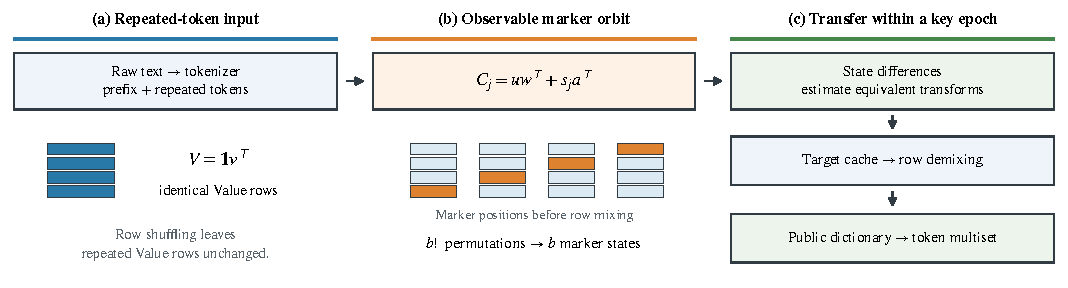
\includegraphics[width=\textwidth]{overview.pdf}
\caption{Attack mechanism. A legal repeat run makes first-layer Value rows identical. Fresh permutations move only the marker, producing a small orbit. The attacker recovers equivalent transforms from its own protected blocks, then matches demixed victim rows against a public-model dictionary. The diagram is schematic; no victim plaintext or server secret is an attack input.}
\label{fig:overview}
\end{figure*}

\section{System and Threat Model}
\label{sec:model}
\subsection{Cache representation and the tested transform}
A decoder stores Key and Value vectors for previously processed tokens. For the first Value layer of the evaluated models, write
\begin{equation}
 v(t)=W_V\,N(E[t])+\beta_V,
 \label{eq:dictionary}
\end{equation}
where $E$ is the public embedding table, $N$ is the first layer's input normalization, and $W_V,\beta_V$ are the relevant head's projection and bias. The implementation detects the appropriate normalization/projection path for each model. Equation~\eqref{eq:dictionary} does not assert that deeper-layer states depend only on the token. It also does not apply to every possible architecture with absolute position-dependent inputs.

Let $V\in\R^{b\times d}$ contain one head's $b$ Value rows. The official default obfuscation path can be written as
\begin{equation}
 C=S P(VM+A),\qquad A=e_r a^\T.
 \label{eq:cloak}
\end{equation}
Here $S\in O(b)$ is a secret orthogonal row transform, $M\in O(d)$ is a structured column transform, $P$ is a block-specific permutation, and $A$ adds a secret vector $a$ to one row. The marker vector is positive in the evaluated configuration. For a fixed head and branch, $S$, $M$, and $a$ are reused by a cloak instance. The marker's effective location changes under $P$. The implementation also exposes optional positive scaling factors; our exact derivation first addresses the default orthogonal configuration, and we evaluate one scaled configuration separately.

The implementation pairs coordinate $i$ with $i+d/2$ in $M$. Each pair is rotated independently. This structure is consequential: recovering an arbitrary $d$-dimensional orthogonal matrix from one vector pair would be underdetermined. We do not make that claim. Rotary position embeddings motivate structured transforms in the original design~\cite{kvcloak,rope}; the implementation uses the paired structure on the Value branch as well.

\subsection{Attacker capabilities}
The adversary knows the original public model and tokenizer. It can submit its own text requests and read the corresponding protected cache blocks. It can also observe a target request's protected cache under the same relevant secret configuration. This observation may model an untrusted cache reader or a cache disclosure, but obtaining that access is outside our attack. A successful experiment does not show that an arbitrary remote API client can read another user's cache.

The adversary does not receive $S$, $M$, $a$, victim plaintext, or the defender's fused model weights. A public local model supplies the dictionary and the plaintext vector for the attacker's own probe. Defender secrets may be used by evaluation-only diagnostics, but are not inputs to the recovery routine. The isolated fused experiment reloads the original model for the attacker and computes its transformed dictionary using recovered parameters.

We assume public block size and head layout. The adversary may calibrate and attack only within a secret epoch shared by probe and target. Instance routing, per-tenant key scopes, or request-specific transformations can prevent that sharing. We do not establish how often real deployments satisfy this condition. The measured lifecycle experiment is a controlled simulation of the shared-secret setting.

\subsection{Goals and exclusions}
The primary goal is recovery of the token multiset in each complete target block. A secondary goal is identifying a synthetic value from an explicitly supplied same-type candidate set. The second goal is conditional on that candidate knowledge; it is not unconstrained recovery of an arbitrary credential.

The experiments do not establish within-block ordering, whole-prompt exact match, deeper-layer recovery, or inference on an untrusted accelerator with unrestricted access to all intermediate computation. We also distinguish floating-point precision: model forward passes are FP32 in the main suite, while cloak matrix operations use bf16. This is not an end-to-end bf16 serving benchmark.

\begin{table}[t]
\centering
\caption{Information boundary used by the attack.}
\label{tab:boundary}
\begin{tabular}{p{.45\columnwidth}p{.41\columnwidth}}
\toprule
Available to attacker & Evaluation only / unavailable \\
\midrule
Original model and tokenizer & Secret configuration \\
Own text and protected probe & Victim plaintext and token labels \\
Protected target blocks & Defender's fused dictionary \\
Public block/head dimensions & True per-block permutation \\
Supplied candidates (value task) & True candidate index for scoring \\
\bottomrule
\end{tabular}
\end{table}

\section{From Permutation Count to Observable Orbit}
\label{sec:analysis}
The analysis separates three questions: how many states can a chosen input produce; whether those states identify reusable parameters; and how many blocks are required to observe them. A large permutation group alone answers none of these questions.

\subsection{Input symmetry collapses the orbit}
Suppose a legal input produces $V=\ones v^\T$. Every row permutation then satisfies $PV=V$. Define $w=M^\T v$ and $u=S\ones$. Equation~\eqref{eq:cloak} becomes
\begin{equation}
 C(P)=u w^\T+S P A.
 \label{eq:orbit}
\end{equation}
Only the marker moves. Identical rows, rather than rank one alone, are essential: a general rank-one matrix $xv^\T$ need not be invariant when the entries of $x$ differ.

\begin{proposition}[Marker orbit]
For fixed $V=\ones v^\T$, fixed $A,M$, and invertible $S$, the number of distinct exact-arithmetic ciphertexts under all row permutations is
\begin{equation}
 |\{C(P):P\in\mathcal S_b\}|=\frac{b!}{|\Stab(A)|},
 \label{eq:stabilizer}
\end{equation}
where $\Stab(A)=\{P:PA=A\}$. For $A=e_ra^\T$ with $a\ne0$, this number is $b$.
\end{proposition}
\begin{proof}
Adding the constant $uw^\T$ and multiplying by invertible $S$ preserve equality of outputs. Thus two outputs agree exactly when their permuted markers agree. The orbit--stabilizer identity gives~\eqref{eq:stabilizer}. A single nonzero marker row can occupy $b$ distinct positions.
\end{proof}

For $k$ identical nonzero marker rows and $b-k$ zero rows, the count is $\binom bk$. If all marker rows are identical, it is one even though the marker has full support. If the $k$ nonzero rows are distinct and different from zero, the count is $b!/(b-k)!$. These examples prevent a misleading sparse-versus-dense dichotomy: marker support size alone does not determine security. Our implemented recovery routine uses the single-row case, not an attack on every orbit in~\eqref{eq:stabilizer}.

In that case, let $s_j=Se_j$. The $b$ ideal states are
\begin{equation}
 C_j=uw^\T+s_j a^\T,\qquad j=1,\ldots,b.
 \label{eq:state}
\end{equation}
Fresh $P$ remains present in the implementation. The attack neither predicts its random seed nor forces it to repeat. Instead, many permutations have the same effect on the chosen input.

\subsection{Identification from the state geometry}
The next result describes an equivalent demixer, not the original order of $S$'s columns.

\begin{theorem}[Default-configuration identification]
\label{thm:identification}
Assume all states in~\eqref{eq:state} are available; $S$ is orthogonal; $a$ is nonzero with known positive orientation; $v$ is known; and $w$ has a nonzero component orthogonal to $a$. Assume further that the known norm $\|w\|=\|v\|$ distinguishes the two signs of $u$. Then $a,w,u$ and the columns of $S$ are identifiable, with the columns unordered. If $M$ consists of independent two-dimensional rotations and the restriction of $v$ to every pair is nonzero, $M$ is identifiable modulo full rotations.
\end{theorem}
\begin{proof}
For $i\ne j$,
\begin{equation}
 C_i-C_j=(s_i-s_j)a^\T.
 \label{eq:rankone}
\end{equation}
This matrix has rank one. Its right singular direction identifies $a/\|a\|$ up to sign; positivity fixes the orientation. Since distinct orthonormal columns satisfy $\|s_i-s_j\|=\sqrt2$, its nonzero singular value is $\sqrt2\|a\|$, identifying the magnitude.

Let $Q_a=I-aa^\T/\|a\|^2$. Then $C_jQ_a=u(Q_aw)^\T$ is a nonzero rank-one matrix. Its left direction identifies $u$ up to sign, and $\|u\|=\sqrt b$ fixes its magnitude. For either sign candidate, use $u^\T s_j=1$ to compute
\begin{equation}
 w^\T=\frac{u^\T C_j-a^\T}{b}.
 \label{eq:w}
\end{equation}
The assumed norm separation selects the correct sign. Each column follows from
\begin{equation}
 s_j=\frac{(C_j-uw^\T)a}{\|a\|^2}.
 \label{eq:s}
\end{equation}
The state labels do not identify the original column indices, leaving an arbitrary column permutation. Finally, within every nonzero coordinate pair, the angle from the known $v$ pair to the recovered $w$ pair identifies the corresponding rotation under the implementation's convention.
\end{proof}

The qualifications are substantive. Choosing $-u$ in~\eqref{eq:w} gives $w'=-w-2a/b$, not merely a harmless sign flip. The norm test fails to distinguish signs precisely when $\langle w,a\rangle=-\|a\|^2/b$. Similarly, a zero pair in $v$ cannot reveal that pair's rotation. A different legal probe may resolve these degeneracies, but our theorem does not promise that one arbitrary token always suffices. Nor does it extend one-pair identification to a general orthogonal $M$.

\subsection{Collection cost and finite precision}
If each block independently maps the marker uniformly to a row, collecting all $b$ states is a coupon-collector process. The expected block count is $bH_b$, with $H_b=\sum_{i=1}^b1/i$. For $b=16$, this is about 54.1 blocks. A union bound gives
\begin{equation}
 \Pr[\text{some state missing after }n]\le b(1-1/b)^n
 \le be^{-n/b}.
 \label{eq:collection}
\end{equation}
For $H$ heads, $n\ge b\log(bH/\delta)$ suffices for the analogous union-bound failure probability $\delta$. Heads need not be independent for this union bound; blockwise sampling within each head must satisfy the premise. Prefixes and padding reduce the number of usable blocks. A count of observed clusters is a calibration diagnostic, not a guarantee of success within a fixed budget or after the key has changed.

Floating-point implementations need not produce identical bit patterns for permutations in the same ideal state. Different accumulation orders can create nearby realizations. If every observed block is within Frobenius distance $\epsilon$ of its ideal state, within-state distances are at most $2\epsilon$. For distinct states, orthogonality gives
\begin{equation}
 \|C_i-C_j\|_F=\sqrt2\|a\|.
\end{equation}
Consequently a separating distance threshold exists whenever $4\epsilon<\sqrt2\|a\|$. This sufficient condition explains why rounding variants can remain clusterable; it is not an asserted error bound for every hardware backend. The experiments measure recovery under the actual bf16 cloak operations instead of inferring it solely from ideal arithmetic.

For dictionary decoding, suppose the true normalized vector $z$ has margin $\gamma$ over every incorrect normalized dictionary vector in inner product, and the recovered normalized vector differs from $z$ by at most $\eta$ in Euclidean norm. Each score changes by at most $\eta$, so $2\eta<\gamma$ suffices to preserve its nearest neighbor. This conditional statement does not cover selecting the correct marker hypothesis, and it does not replace measurements of dictionary ambiguity. We make no uniform numerical-margin claim across the vocabulary.

\section{Attack Construction}
\label{sec:attack}
\subsection{Reachable probes and state recovery}
The attack searches a small character set for text whose normal tokenization contains a sufficiently long constant-token run. It submits the tokenizer's complete output, including any beginning-of-sequence or other prefix tokens. If the run begins at token offset $p$ and the input contains $L$ tokens, the usable block indices are
\begin{equation}
 \left\lceil p/b\right\rceil,\ldots,\left\lfloor L/b\right\rfloor-1.
\end{equation}
This filtering happens on the attacker side. It does not remove the prefix before the model computes its cache. The main suite records the probe text character, prefix length, total token count, and whether this raw-entry path succeeded. All twelve included configurations use that path.

For each head, the attacker flattens protected probe blocks, groups nearby states, and computes a representative for each group. It then estimates the rank-one directions in~\eqref{eq:rankone}, aligns their signs, and combines them to estimate $a$. Projection orthogonal to that direction yields $u$; the known public probe vector selects its sign. Equations~\eqref{eq:w} and~\eqref{eq:s} recover the remaining parameters. The implementation checks state coverage before attempting recovery. Ground-truth column similarities are evaluation diagnostics, not decisions supplied to the attack.

Let $\widetilde S$ contain the recovered columns in state order. In exact arithmetic, $\widetilde S=S\Pi$ for some unknown permutation $\Pi$. Then $\widetilde S^\T S=\Pi^\T$. This unordered recovery is sufficient for content extraction: it only changes the order in which recovered rows are returned.

\subsection{Decoding an unseen block}
For each protected target block $C$, the attacker enumerates the $b$ possible marker columns. For hypothesis $j$, it forms
\begin{equation}
 Y_j=\widetilde S^\T(C-\widetilde s_j a^\T)\widehat M^\T.
 \label{eq:decode}
\end{equation}
Under the correct marker hypothesis and exact recovery, $Y_j$ is a row-permuted copy of $V$. For each row, the attacker selects the nearest normalized vector from the dictionary in~\eqref{eq:dictionary}. It chooses the marker hypothesis with the largest sum of rowwise best-match cosine scores. This final selection is a measured heuristic; the identification theorem does not by itself guarantee its success for every vocabulary and block.

The output preserves multiplicity but not within-block order. We score it by multiset intersection:
\begin{equation}
 \operatorname{hit}(\widehat T,T)=\sum_t\min\{n_{\widehat T}(t),n_T(t)\}.
 \label{eq:metric}
\end{equation}
The denominator is $b$ per scored head and block. Repeated observations of the same token across heads remain separate evaluation opportunities; they are not independent textual samples.

The dictionary is a one-time public-model computation. Calibration uses state clustering and small-matrix factorizations. Target recovery tries $b$ marker hypotheses and performs rowwise dictionary comparisons. Thus the attack does not enumerate $b!$ permutations. Its practical cost still depends on vocabulary size, dimension, and implementation of nearest-neighbor search. We do not present a deployment-throughput claim from the current CPU scripts.

\subsection{Fusion, scaling, and secret scope}
In fused mode, the server folds $M$ into its projection weights, producing $VM$ before the cache obfuscator. The attacker still uses its unfused public model. It recovers the corresponding transformed probe vector from protected states and composes the public dictionary with $\widehat M$. Our isolated experiment uses independent public and defender model objects; the earlier shortcut of constructing an attack dictionary from fused defender weights is excluded from its reported result.

The optional scaling configuration changes orthogonal matrices into structured rotation/scaling transforms. It requires modified recovery equations rather than an unqualified application of Theorem~\ref{thm:identification}. We include its recorded behavior as a separate implementation variant. The exact theorem applies to its stated orthogonal setting only.

Parameters are recovered for a head and secret epoch. A new permutation does not invalidate them; a new secret transform may. This distinction is tested by applying recovered parameters to fresh requests under the same configuration, to a new configuration as a negative control, and to a refreshed configuration after recalibration. Those tests isolate parameter reuse from a claim that the attack survives arbitrary key rotation.

\section{Evaluation}
\label{sec:evaluation}
We ask four questions. \textbf{RQ1} tests whether legal repeated-token inputs produce the predicted small orbit and identify an equivalent demixer. \textbf{RQ2} measures token-multiset recovery across models and configurations. \textbf{RQ3} tests the official entry point and the effect of secret lifetimes. \textbf{RQ4} asks whether the recovered content supports a concrete, bounded privacy task and whether shortening the secret lifetime interrupts transfer.

\subsection{Experimental methodology}
\label{sec:methodology}
The main suite uses the official \scheme{} implementation at commit \texttt{6b40f36}. We do not modify its cache transformation. Model forward passes use FP32 weights on CPU, and the cloak stores/transforms cache blocks in bf16, matching the implementation default. Experiments ran on an AMD EPYC 9554 host. Table~\ref{tab:breadth} reports ten distinct public models from the Qwen, Llama, OLMo, Phi, and TinyLlama families~\cite{qwen25,llama3,olmo,phi3,tinyllama} and twelve configurations; Qwen2.5-0.5B additionally covers block sizes 8 and 32. Checkpoint revisions are listed in Appendix~\ref{app:repro}.

For every configuration, the attacker submits text through the unmodified tokenizer. Any beginning-of-sequence or other prefix token remains in the model input. Calibration uses only complete blocks inside the final constant-token run; content recovery is scored on complete blocks of the target texts. Calibration requires all $b$ states to be observed for a head. Every head in the main suite calibrated, so Table~\ref{tab:breadth} includes all heads.

Five target texts cover English prose, Python, Chinese, dialogue, and mathematical prose. Each is evaluated under two fresh block-permutation seeds. The primary metric is the multiset hit count in~\eqref{eq:metric}, summed over complete blocks and calibrated heads. Thus a ``head--token opportunity'' is one token position scored through one KV head. Opportunities within a document, across heads, and across seeds are correlated. We report their raw descriptive total and per-configuration rates; we do not use a token-level binomial interval as evidence of generalization to independent requests.

The main-suite fresh-secret control applies a demixer calibrated under one complete configuration to a cache produced under another, scoring head 0 on the English prose target. Its denominator therefore differs from the multi-head, five-text primary metric. Ground-truth secrets are used only for diagnostics such as parameter similarity. The attack routine receives the public model, its own protected calibration cache, and protected target blocks.

\paragraph{Configuration and input accounting}
The main runner estimates the defender's magnitude thresholds from eight fixed natural-language sentences stored separately from the five target texts. It generates one secret configuration per model/block-size cell with seed 42, then evaluates two target-cache permutation seeds, 5001 and 5002. These two seeds change the block permutations; they do not constitute two independently generated secret configurations. The additional multi-epoch study below varies the complete configuration and answers a different question.

Probe lengths are recorded after tokenization. Character repetition can produce different token counts across tokenizers, and the search may overshoot its target length. The table therefore reports the actual submitted token count rather than a nominal character or token budget. Prefix lengths are one token for the recorded Llama and Phi configurations and two for TinyLlama; the remaining main-suite configurations have no prefix before the constant-token run. Prefix-containing blocks and incomplete final probe blocks are excluded from calibration. Target texts are independently truncated to their last complete block, so the reported recovery denominator excludes their trailing partial blocks.

These choices define the unit of each result. The main table aggregates head--token opportunities under the fixed texts and recorded configurations. The probe curve measures repeated calibration trials, the epoch study averages session rates under new configurations, and the privacy study ranks a supplied candidate set. Their denominators are not interchangeable: adding their reported successes into one grand total would mix different questions and levels of aggregation.

\subsection{RQ1: orbit and parameter recovery}
Every evaluated head forms exactly $b$ clusters after prefix blocks are removed: 8, 16, or 32 according to the configuration. The smallest saved between/within cluster-separation ratio is 500.2. Evaluation matches recovered columns of $S$ to true columns by cosine similarity and checks that the matching is bijective. The minimum matched cosine similarity is 0.999996; the largest relative error recorded for $w$ is 0.0354. These evaluation-only diagnostics support the predicted rank-one state geometry.

Figure~\ref{fig:probe} compares the observed two-head calibration rate on Qwen2.5-0.5B with the exact one-head occupancy probability for independent uniform states. Each empirical point contains ten trials under one fixed secret configuration. This diagnostic counts a trial as successful when both heads collect all states and the recorded marker and minimum matched-column cosine similarities each reach 0.999. With 80 blocks (1,280 repeated tokens), 9/10 trials meet this criterion; with 128 blocks (2,048 tokens), all ten do. The small, independently seeded trial sets can yield a non-monotone empirical curve. The comparison supports the coupon-collector scale rather than estimating a deployment success curve.

\begin{figure}[t]
\centering
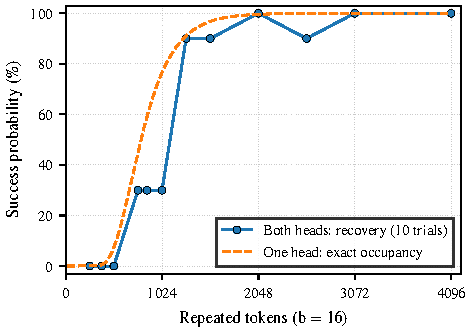
\includegraphics[width=\columnwidth]{probe_budget.pdf}
\caption{Calibration versus probe length for $b=16$. The empirical series requires full recovery of both heads; the dashed series is the exact one-head occupancy probability. Ten trials are used at each empirical budget.}
\label{fig:probe}
\end{figure}

\subsection{RQ2: content recovery}
Across the twelve configurations in Table~\ref{tab:breadth}, the attack obtains 263,029 hits in 263,904 head--token opportunities, or 99.668\%. Per-configuration recovery ranges from 99.318\% on Phi-3-mini to 100\% on six configurations. Fresh-secret control recovery ranges from 0 to 0.625\%: ten configurations have zero hits, while the $b=8$ and $b=32$ configurations each have one hit. These controls support the role of the recovered secrets in the observed recovery.

\begin{table*}[t]
\centering
\caption{Main-suite recovery from first-layer Value caches. ``Probe'' is the complete tokenizer output length; C/N is the raw multiset hit count. The control uses a fresh secret configuration.}
\label{tab:breadth}
\setlength{\tabcolsep}{3.5pt}
\begin{tabular}{lrrrrrrr}
\toprule
Model & $b$ & Heads & $d$ & Probe & C/N & Rec. (\%) & Control \\
\midrule
Llama-3.2-1B & 16 & 8 & 64 & 3,201 & 20,192/20,224 & 99.84 & 0/176 \\
OLMo-2-1B & 16 & 16 & 128 & 3,200 & 45,043/45,056 & 99.97 & 0/176 \\
Phi-3-mini & 16 & 32 & 96 & 4,080 & 111,872/112,640 & 99.32 & 0/208 \\
Qwen2.5-0.5B & 16 & 2 & 64 & 3,200 & 4,800/4,800 & 100.00 & 0/176 \\
Qwen2.5-0.5B & 32 & 2 & 64 & 20,250 & 4,608/4,608 & 100.00 & 1/160 \\
Qwen2.5-0.5B & 8 & 2 & 64 & 1,280 & 4,896/4,896 & 100.00 & 1/176 \\
Qwen2.5-1.5B & 16 & 2 & 128 & 3,200 & 4,768/4,800 & 99.33 & 0/176 \\
Qwen2.5-3B & 16 & 2 & 128 & 3,200 & 4,800/4,800 & 100.00 & 0/176 \\
Qwen2.5-7B & 16 & 4 & 128 & 3,200 & 9,578/9,600 & 99.77 & 0/176 \\
Qwen3-0.6B & 16 & 8 & 128 & 3,200 & 19,200/19,200 & 100.00 & 0/176 \\
Qwen3-1.7B & 16 & 8 & 128 & 3,200 & 19,200/19,200 & 100.00 & 0/176 \\
TinyLlama-1.1B & 16 & 4 & 64 & 2,033 & 14,072/14,080 & 99.94 & 0/208 \\
\midrule
\multicolumn{5}{r}{Total} & 263,029/263,904 & 99.668 & -- \\
\bottomrule
\end{tabular}
\end{table*}

We separately exercise two implementation variants whose records do not share the main table's denominator. In the fused path, an isolated attacker instance uses the original public model and recovered transform; it does not read the defender's fused weights. Recovery is 100\% on each of the English, Chinese, and Python targets tested. In the optional \texttt{need\_ratio} path ($S$ and $M$ ratio 1.25), the variant-specific recovery succeeds on all five target texts and both permutation seeds. These results establish reachability for the tested variants, not coverage of their full parameter spaces.

\paragraph{Where the misses occur}
The main total contains 875 missed head--token opportunities. Phi-3-mini contributes 768 of them and also has the largest denominator, 112,640, because its first Value layer has 32 KV heads. Its per-configuration recovery remains 99.318\%. This concentration cautions against reading the aggregate as an equal-weight average over models: both the number of heads and the tokenized text lengths affect a configuration's weight.

Table~\ref{tab:textcounts} regroups the same raw counts by target text. It introduces no additional samples. Each row represents one fixed text evaluated repeatedly across configurations, heads, and the two permutation seeds; it is not an estimate over a language or application domain. The breakdown shows that the aggregate is not supplied by one text alone. It cannot establish, for example, that Chinese is easier to recover than English, since vocabulary, length, content, and model weighting all differ.

\begin{table}[t]
\centering
\caption{The main-suite counts regrouped by fixed target text. These are the same correlated evaluation opportunities as Table~\ref{tab:breadth}, not additional experiments.}
\label{tab:textcounts}
\begin{tabular}{lrr}
\toprule
Target text & Matches / opportunities & Misses \\
\midrule
English prose & 33,795 / 33,920 & 125 \\
Python code & 58,587 / 58,784 & 197 \\
Chinese prose & 80,517 / 80,768 & 251 \\
Dialogue & 37,928 / 38,048 & 120 \\
Mathematical prose & 52,202 / 52,384 & 182 \\
\midrule
Total & 263,029 / 263,904 & 875 \\
\bottomrule
\end{tabular}
\end{table}

The retained counters do not identify the cause of each miss. Finite-precision parameter error, marker-hypothesis selection, and dictionary ambiguity are possible explanations, but these aggregates cannot attribute their relative contributions. In particular, a high cosine similarity for recovered parameters does not imply exact token recovery when dictionary margins are small. The conditional margin argument in Section~\ref{sec:analysis} describes that dependency without assigning a measured cause to unretained per-block errors.

The evaluated Value-only attack outputs token multisets. An exploratory ordering script records 9.1\% and 15.9\% position accuracy on 11 blocks with Qwen2.5-0.5B and Qwen2.5-3B, respectively, and no exact blocks. However, it passes unique token keys to beam search and drops multiplicity. Its 6.25\% reference also assumes distinct positions without accounting for repeated token identities. We retain these exploratory observations for transparency but draw no conclusion about the difficulty of order recovery from them.

\subsection{RQ3: entry point and secret lifetime}
\paragraph{Official entry point}
We construct the directory layout expected by the authors' command-line pipeline, invoke their configuration generator and obfuscator, and attack the protected files they produce. The targets are 16 English conversations selected from a public LMSYS-Chat-1M mirror~\cite{lmsys}. The defender's magnitude thresholds are computed from the first eight target conversations; this setup is not an independent calibration/test split. Target plaintext is not supplied to the recovery routine. The saved per-file rates are 100\% for all 16 files. This record supports a controlled file-format test, not a production-service or remote-access claim. The historical harness reused an output directory and did not enforce subprocess success before reading files, so the saved summary alone does not certify a fresh end-to-end execution.

\paragraph{Multiple secret epochs}
Figure~\ref{fig:epochs} summarizes three models and five independently generated configurations per model. All heads calibrate in all 15 model--epoch cells. Mean recovery across epoch means is 100\% for Qwen2.5-0.5B, 99.64\% for Llama-3.2-1B, and 99.34\% for Phi-3-mini; the lowest model-level epoch mean is 99.29\%. Wrong-secret controls average 0.05\%, 0.01\%, and 0.16\%, respectively. The same ten public conversations recur across epochs and overlap earlier public-data experiments, so we treat this as secret-epoch stability, not held-out-session generalization. The result file retains rounded session rates rather than raw counts.

\begin{figure*}[t]
\centering
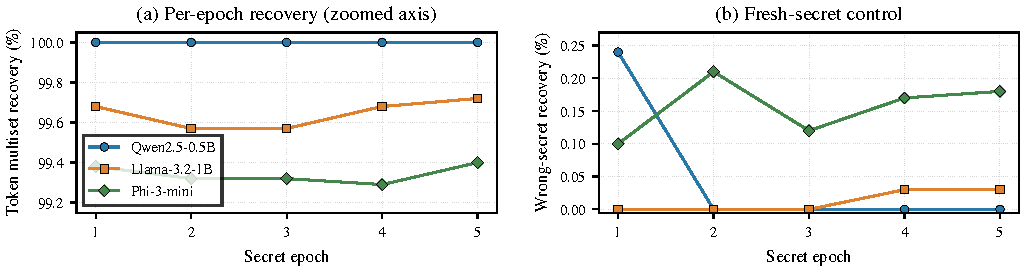
\includegraphics[width=.88\textwidth]{key_epochs.pdf}
\caption{Secret-epoch stability on three models. Every epoch calibrates all heads. The y-axis in (a) is deliberately zoomed; (b) uses demixers from the wrong configuration. The conversations are not an exclusive held-out set.}
\label{fig:epochs}
\end{figure*}

\paragraph{Lifecycle simulation}
In a controlled Qwen2.5-0.5B service simulation, one calibration request is followed by ten synthetic requests from different application domains. Recovery is 100\% on all ten. Replacing the complete secret configuration reduces a stale demixer to 0.78\%; one new calibration probe restores 100\% on the measured request. This result identifies the relevant unit of exposure: a shared secret epoch. It does not estimate tenant co-location prevalence in real deployments.

The lifecycle and epoch experiments support different interpretations of reuse. Recalibrating after rotation shows that a new shared epoch can again supply the same type of calibration opportunity; it does not mean the old demixer survives rotation. The separate request-refresh experiment asks whether an old demixer transfers when its row secrets are no longer shared. Reporting both observations makes the scope of the proposed intervention explicit.

\subsection{RQ4: bounded privacy consequence}
We evaluate closed-set identification on 30 synthetic cases. For each of six value types---SSN-like strings, card numbers, passwords, medical record numbers, names, and addresses---we generate a fixed list of 100 candidates and use the first five as truths. A target value is embedded in neutral context. The attacker aggregates recovered tokens from all complete blocks and all heads; it is not told which block contains the value. A candidate is scored by the fraction of its unique tokens present in the recovered multiset.

Let $g$ be the number of candidates with a strictly higher score than the truth and $m$ the size of the truth's tie group. The truth attains the maximum in all 30 cases ($g=0$); it is the unique maximum in 21/30. Under uniform random tie-breaking within the recorded group, expected top-1, top-5, and top-10 success are 77.36\%, 90.95\%, and 95.24\%, respectively. Uniform guessing from 100 candidates gives 1\%, 5\%, and 10\%. Figure~\ref{fig:privacy} shows the top-1 result by value type.

The expected top-$k$ contribution of a case is
\begin{equation}
 p_k(g,m)=\min\{1,\max\{0,(k-g)/m\}\}.
 \label{eq:ties}
\end{equation}
There are $g$ candidates ahead of the tie group and $m$ equally likely positions within it. If the remaining top-$k$ slots cover the entire group, success is one; otherwise the fraction of covered positions determines the expectation. Thus $g=0$ means that the truth is not outranked, whereas unique identification additionally requires $m=1$. We average these per-case expectations over the 30 retained cases, rather than treating tied maxima as deterministic successes.

The candidate score tests token membership, not order or a verified field span. A candidate can share tokens with the surrounding context or with another candidate. Even perfect recovery of a target multiset can therefore leave several values tied. Conversely, identifying a candidate from a supplied list does not imply that the method can generate that value without candidate knowledge. These distinctions explain why the privacy outcome and the main multiset metric are complementary rather than interchangeable.

\begin{figure}[t]
\centering
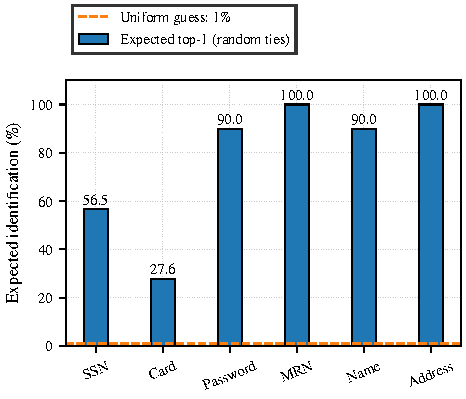
\includegraphics[width=\columnwidth]{privacy.pdf}
\caption{Closed-set identification in the 30-case synthetic study. Each bar contains five cases. Ties are broken uniformly in expectation.}
\label{fig:privacy}
\end{figure}

This experiment is evidence of consequence, not a population estimate. Truths are the first five generated candidates rather than uniform random indices; the displayed 1\% line is therefore a uniform-guess reference, not a matched optimal prior. Only the truth score and $(g,m)$ summaries were retained, not all candidate scores or recovered multisets. An ``entity complete'' flag used a token-set approximation rather than a verified character span. We consequently do not claim unconstrained credential recovery, stable per-type rates, or complete-field reconstruction.

\subsection{Shortening the secret lifetime}
The mechanism suggests refreshing the reused row transform $S$ and marker $a$ while leaving the fused column transform $M$ static. In one Qwen2.5-0.5B experiment, the saved same-epoch recovery rate is 97.44\%, compared with 0\% when a demixer calibrated for request A is applied after $S,a$ are regenerated for request B. The result JSON retains rounded rates rather than raw counts for this comparison. Generating the corresponding matrices for the full model takes 2.9\,ms in a CPU microbenchmark.

This is a mitigation candidate, not a validated repair. The saved round-trip check does not establish full K/V functional equivalence, and the test does not cover adaptive within-request calibration, shared prefixes, multi-turn identity, device-transfer cost, or end-to-end serving latency. The defensible conclusion is narrower: request-specific $S,a$ prevents the \emph{existing} cross-request demixer from transferring in the measured setting.

\subsection{Answers to the research questions}
The observed state counts and parameter errors support the predicted marker orbit (RQ1). Recovery is high across the tested models and configurations, while fresh-secret control recovery remains between 0 and 0.625\% (RQ2). The attack consumes the official protected-cache output and remains effective across generated secret epochs, provided calibration and target caches share the relevant secrets (RQ3). The synthetic closed-set study exceeds the uniform-guess reference, with candidate selection and incomplete traces limiting its interpretation. Shortening the row-secret lifetime interrupts the measured transfer, but functional correctness and general security remain unverified (RQ4).

\section{Discussion}
\label{sec:discussion}
\subsection{The security lesson: observable entropy}
The failure is not that the implementation forgets to sample a permutation. It samples one for each block. The failure is that, for a reachable input symmetry, many sampled permutations become observationally equivalent. The security-relevant quantity is the orbit of the transformed object, not the cardinality of the randomizer's support. A $b!$ implementation choice can therefore contribute only $b$ distinguishable calibration states.

This distinction is broader than \scheme{}, but the attack is not a theorem about all linear obfuscation. A designer must ask which transformations survive after quotienting by input stabilizers, which fixed structure remains across observations, and whether recovery metadata becomes an oracle. In the tested construction, the single-row marker is both necessary for legitimate inversion and the label that exposes the columns of $S$. Different marker or mixing structures can change the orbit and the identification problem.

\subsection{Mitigation implications}
Three principles follow. First, do not reuse a transform merely because another component is refreshed: the refreshed component may vanish under a chosen input. Second, bind secrets to the smallest practical identity---request, tenant, or cache object---and specify how shared prefixes and multi-turn sessions inherit that identity. Third, evaluate functional recovery and security together. Replacing a sparse marker with a denser object can defeat this decoder while also breaking the intended inverse; failure of the current attack is not evidence of a correct defense.

Request-specific $S,a$ is the simplest intervention suggested by our measurements. It changes the attacker's problem from amortizing one calibration over other requests to calibrating within the victim's secret scope. Yet the correct engineering choice may instead be authenticated encryption when caches are only stored or transported and need not be manipulated while protected. Obfuscation should be justified by an operation that conventional cryptography cannot efficiently support, not by a general claim that transformed vectors are unintelligible.

\subsection{Limitations and external validity}
Our attacker begins after protected-cache observation is available. We do not show a remote API path to another tenant's cache, measure the prevalence of shared secret epochs, or bypass access control. The study concerns the first Value layer and the tested public implementation. Deeper states, Key recovery, architectures with position-dependent Value inputs, arbitrary orthogonal $M$, and marker patterns outside the analyzed orbit require separate arguments.

The output is unordered within a block. A multiset can expose rare values or keywords, but it is weaker than a verbatim prompt. The synthetic value study uses one model, one secret configuration, 30 cases, and an artificial candidate set. Its incomplete retained traces rule out post-hoc analyses that would require all scores or recovered blocks. The official-entry and multi-epoch studies reuse public conversations; neither supports a claim about an unseen deployment distribution.

The main 99.668\% total weights models with more KV heads and texts with more complete blocks more heavily. It is an audit total, not an estimate over a defined population of users. The model and checkpoint breadth nevertheless tests whether the mechanism is tied to one tokenizer or hidden dimension. Claims about prevalence, per-user harm probability, and production cost remain outside the evidence.

\subsection{Ethics, disclosure, and release}
All experiments ran locally on public model checkpoints, synthetic text, or a publicly released conversation dataset~\cite{lmsys}. We did not recruit or interact with human participants, query a live third-party service, access private caches, or recover non-public user data. No separate human-subjects protocol was submitted because the study involved no participant interaction or new private-data collection. The public conversation subset is used only to exercise file-format and recovery behavior; the manuscript does not reproduce conversation text or identifiers.

The attack is dual use because cache-read access could be converted into content leakage. The authors of \scheme{} were notified of this vulnerability via a GitHub issue on September 28, 2026. The public notice requested a private reporting channel and did not disclose the technical details. We are awaiting a response and will coordinate the detailed disclosure and release timeline with the maintainers. Until affected parties have had a reasonable opportunity to respond, a public artifact should prioritize the proof, frozen aggregate evidence, and inert synthetic reproduction over turnkey integration with live services. No external message is sent by the artifact build process.

We will release an anonymized artifact containing the source snapshot, hashes of frozen result records, figure/table generation, and local synthetic examples, subject to the disclosure timeline. The artifact will distinguish exploratory files from the records supporting paper claims. Any change to a frozen result or denominator will require regenerating the evidence manifest and manuscript assets.

\section{Related Work}
\label{sec:related}
\begin{table*}[t]
\centering
\caption{Closest attack mechanisms. ``Refresh'' describes the component relevant to the cited attack, not every randomness source in the system.}
\label{tab:neighbors}
\setlength{\tabcolsep}{4pt}
\begin{tabular}{>{\raggedright\arraybackslash}p{.17\textwidth}|>{\raggedright\arraybackslash}p{.13\textwidth}|>{\raggedright\arraybackslash}p{.13\textwidth}|>{\raggedright\arraybackslash}p{.17\textwidth}|>{\raggedright\arraybackslash}p{.29\textwidth}}
\TableTop
\rowcolor{TableHead}
\textbf{Work} & \textbf{Protected asset} & \textbf{Attacker input/view} & \textbf{Refreshed structure} & \textbf{Distinguishing step} \\
\TableHeadRule
Hidden No More~\cite{hidden} & hidden states & public model; permuted states & per-scheme permutation & candidate distances reverse the hidden permutation \\
\hline
Partial TEE~\cite{partialtee} & weights and activations & ENCRYPT queries incl. zero and basis vectors & fixed precomputed noise basis & cancel noise subspace; recover permutation and weights \\
\hline
Collapse~\cite{collapse} & obfuscated weights & multiple exposed weight views & low-rank mask, scaling, permutation per epoch & primitive decomposition, rank/overlap tests, alignment \\
\hline
\rowcolor{TableBlue}
This work & runtime Value cache & normal text; protected cache & row permutation per block & input symmetry collapses orbit; marker differences recover equivalent demixer \\
\TableBottom
\end{tabular}
\end{table*}

\subsection{KV-cache and internal-state privacy}
KV caches are central to efficient autoregressive serving; PagedAttention makes fixed-size cache blocks a first-class memory-management unit~\cite{paged}. The same states encode prompt information. Prior work reconstructs text from embeddings and internal activations through optimization, generation, or dictionary search~\cite{morris2023,li2023,dong2025}. \scheme{} demonstrates direct, collision, and injection attacks against unprotected caches, then proposes reversible cache obfuscation~\cite{kvcloak}. We analyze that proposed protection rather than repeating its attacks on plaintext caches.

\subsection{Attacks on permutation and obfuscation defenses}
Hidden No More recovers prompts from permuted hidden states and challenges proofs based on permutation hardness~\cite{hidden}. Saini et al. exploit reuse of precomputed noise bases in partial-TEE systems using chosen internal vectors, recovering secret permutations and weights~\cite{partialtee}. Collapse gives a primitive-level analysis of weight-obfuscation schemes and attacks compositions that retain algebraic structure across refreshed views~\cite{collapse}. These works establish that permutation, linear mixing, and refresh are not independently persuasive security arguments.

Our observation and target differ. The attacker supplies legal text rather than arbitrary hidden vectors; the protected object is a runtime Value cache; an unknown dense row transform remains; and a new row permutation is drawn per block. Repeated text makes the data term invariant, while a sparse recovery marker turns the fresh permutations into a finite-state signal. Table~\ref{tab:neighbors} makes this mechanism-level boundary explicit.

\subsection{Confidential inference and refreshed mixing}
Confidential inference spans secure computation, trusted execution, differential privacy, obfuscation, and hybrids; the recent SoK by Yaluhin compares these families and emphasizes their distinct trust and deployment costs~\cite{sok}. GELO refreshes invertible mixing per batch and explicitly studies Gram leakage, blind-source separation, and shield vectors~\cite{gelo}. ConjFormer instead changes the architecture to be orthogonally equivariant, permitting inference in a rotated basis~\cite{conjformer}. These designs reinforce the importance of refresh scope and of testing invariants exposed by structured transforms.

We do not propose a new general obfuscation system. Our mitigation result is intentionally modest: shortening the lifetime of two reused components prevents the current demixer from transferring in one setting. This preserves the paper's contribution as an attack and analysis, and avoids treating failure of a finite attack battery as a security proof.

\subsection{Positioning relative to the original CPA}
The \scheme{} paper already considers chosen-plaintext attacks on simpler linear constructions and introduces the marker and per-block permutation as part of the hardened design~\cite{kvcloak}. Repeated or low-rank inputs and public-model dictionaries are therefore not, by themselves, new contributions. The difference is retaining the complete published transform and using the marker's \emph{post-permutation orbit} to recover the reusable structure despite a fresh $P$ for every block. Our evaluation accordingly includes the official entry point, fused mode with an isolated public dictionary, fresh-secret controls, and secret-lifetime tests.

This distinction can be stated at the level of the observed matrices. The original paper's naive construction has a fixed linear relation between plaintext differences and ciphertext differences. Its hardened construction inserts a new block permutation, so the original relation cannot simply be assumed to align two arbitrary observations. Our calibration input instead fixes the data term under all row permutations. The variation that remains comes from the marker. The analysis studies this remaining variation directly, without assuming that the sampled permutations are equal or that their labels are known.

Collapse studies exposed weight views with additive masks, scaling, and refreshed permutations~\cite{collapse}. Our protected caches additionally contain dense row mixing that must be identified before dictionary decoding. Repeated-input marker states supply that signal. The distinction concerns the observed matrix structure and input capability; refreshing randomness and linear-algebraic recovery are themselves established topics.

\section{Conclusion}
Fresh randomness is useful only to the extent that it creates fresh observable uncertainty. In \scheme{}, a legal repeated-token request makes the first-layer Value term invariant to row permutations. The remaining marker visits a small orbit whose rank-one differences identify an equivalent demixer. Across ten models and twelve configurations, the attack recovers 263,029 of 263,904 head--token opportunities, while wrong-secret controls remain between 0 and 0.625\%. The attack also consumes the official protected-cache output and transfers across requests within a secret epoch.

The result is strong but bounded: it recovers blockwise token multisets, begins with cache observation, and does not establish deployment prevalence or a complete repair. A limited closed-set study shows why those multisets can matter, while request-specific refresh blocks the tested cross-request transfer without proving general security. The broader design rule is to analyze the observable orbit induced jointly by randomness and reachable inputs. Counting random choices without that quotient can substantially overstate protection.

\clearpage
\bibliographystyle{IEEEtran}
\bibliography{references}
\appendices
\section{Reproducibility Details}
\label{app:repro}
\subsection{Frozen model revisions}
Table~\ref{tab:revisions} records the local Hugging Face revision associated with every distinct checkpoint in the main suite. Qwen2.5-0.5B is reused for the block-size variants and the focused studies.

\begin{table*}[h]
\centering
\caption{Checkpoint identifiers and locally frozen revisions.}
\label{tab:revisions}
\setlength{\tabcolsep}{4pt}
\begin{tabular}{ll}
\toprule
Checkpoint & Revision \\
\midrule
\texttt{Qwen/Qwen2.5-0.5B} & \texttt{060db6499f32faf8b98477b0a26969ef7d8b9987} \\
\texttt{Qwen/Qwen2.5-1.5B} & \texttt{8faed761d45a263340a0528343f099c05c9a4323} \\
\texttt{Qwen/Qwen2.5-3B} & \texttt{3aab1f1954e9cc14eb9509a215f9e5ca08227a9b} \\
\texttt{Qwen/Qwen2.5-7B} & \texttt{d149729398750b98c0af14eb82c78cfe92750796} \\
\texttt{Qwen/Qwen3-0.6B} & \texttt{c1899de289a04d12100db370d81485cdf75e47ca} \\
\texttt{Qwen/Qwen3-1.7B} & \texttt{70d244cc86ccca08cf5af4e1e306ecf908b1ad5e} \\
\texttt{unsloth/Llama-3.2-1B} & \texttt{9535bd9b1d1dea6acafbdc4813b728796aeb28da} \\
\texttt{allenai/OLMo-2-0425-1B} & \texttt{a1847dff35000b4271fa70afc5db10fd29fedbdf} \\
\texttt{microsoft/Phi-3-mini-4k-instruct} & \texttt{f39ac1d28e925b323eae81227eaba4464caced4e} \\
\texttt{TinyLlama/TinyLlama-1.1B-Chat-v1.0} & \texttt{fe8a4ea1ffedaf415f4da2f062534de366a451e6} \\
\bottomrule
\end{tabular}
\end{table*}

The LMSYS cache revision visible during artifact preparation is \texttt{200748d9d3cddcc9d782887541057aca0b18c5da}. The official-entry script used the public mirror \texttt{AarushSah/lmsys-chat-1m}; the saved result contains only truncated hashes and accuracies, not conversation text.

\subsection{Evidence and generated assets}
The artifact separates model-running code from manuscript generation. JSON records under \texttt{paper/evidence/} are copied from the frozen experiment results and listed with SHA-256 hashes in \texttt{manifest.json}. The script \texttt{paper/scripts/generate\_assets.py} reads only those records, regenerates all manuscript figures and an audited copy of the main-table rows, recomputes the reported privacy tie statistics, and asserts the principal denominator 263,029/263,904. The submission checker verifies that every generated row is present verbatim in the manuscript source. Neither script makes a model or network call.

The original runs did not persist a complete Python dependency lock. The artifact therefore freezes source, model revisions, input/result records, and the manuscript-generation environment separately; claims of bit-identical model reruns should not be made without reconstructing the missing runtime versions. This limitation does not affect hash verification or regeneration of paper assets from the frozen records.

\section{Additional Scope Notes}
The official implementation applies the same row permutation to the corresponding K and V blocks, but the present attack and primary metric target first-layer V. An exploratory position-calibration experiment shows that controlled marker/position pairs can label 60/64 blocks per head in one setting, while direct language-model ordering does not recover an exact block. We omit an ordered-reconstruction claim because these observations do not close the K-recovery and numerical-error chain.

For the single-row marker, Theorem~\ref{thm:identification} recovers columns of $S$ as a set. That is enough for multiset decoding: applying an unknown column permutation simply reorders recovered rows. Claims about the original row indices, absolute token positions, or attention semantics would require resolving that labeling and jointly validating K and V.

\end{document}
